\documentclass{article}
\usepackage[utf8]{inputenc}
\usepackage[margin=0.73in]{geometry}
\usepackage{hyperref}
\usepackage{graphicx}
\usepackage{datatool, filecontents}
\DTLsetseparator{,}

\DTLloaddb[noheader, keys={thekey,thevalue}]{texData}{../scripts/texData.dat}
\newcommand{\var}[1]{\DTLfetch{texData}{thekey}{#1}{thevalue}}

\graphicspath{ {../plots/} }
\hypersetup{
    colorlinks=true,
    linkcolor=blue,
    filecolor=magenta,
    urlcolor=cyan,
}

\begin{document}

    \begin{center}

        % MAKE SURE YOU TAKE OUT THE SQUARE BRACKETS

        \LARGE{\textbf{ICC Men's Ranking}} \\
        \vspace{1em}
        \Large{An Auto-generated Report on ICC Men's Ranking} \\
        \vspace{1em}
        \normalsize{Dated: \var{day}-\var{month}-\var{year}}
        \vspace{1em}

    \end{center}

    \vspace{4em}
    \tableofcontents

    \newpage

    \begin{normalsize}

        \section{T20i Format}\label{sec:t20i-format}
            \subsection{Batting}\label{subsec:batting1}
                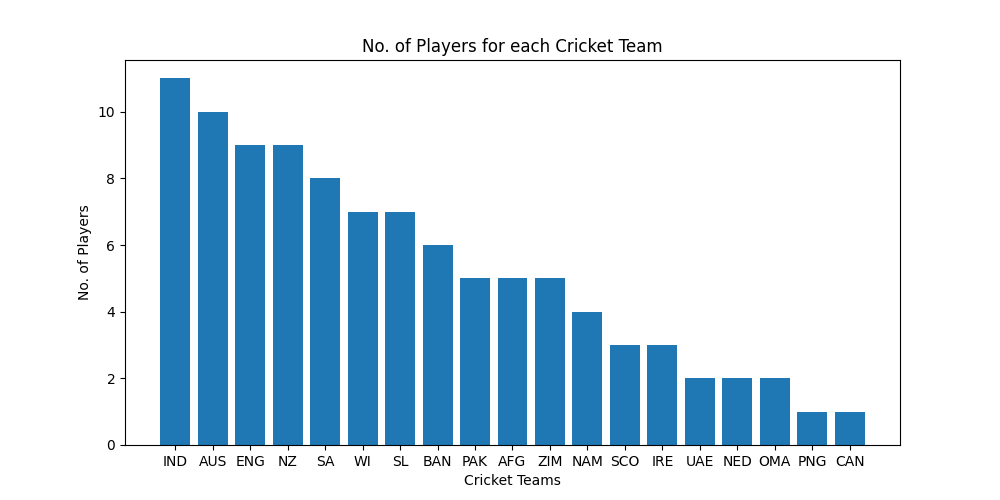
\includegraphics[scale=0.7]{t20i_batting-1}
                \vspace{1em}\\
                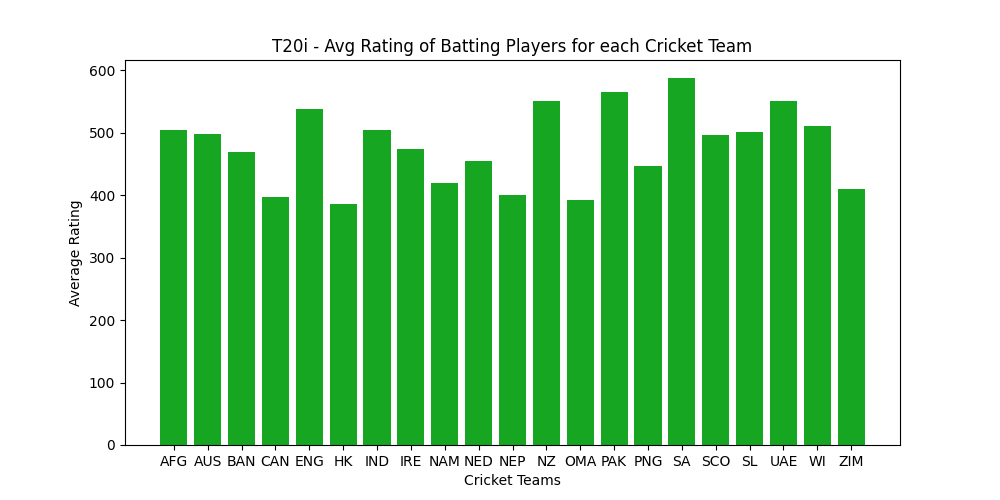
\includegraphics[scale=0.7]{t20i_batting-2}
            \subsection{Bowling}\label{subsec:bowling1}
                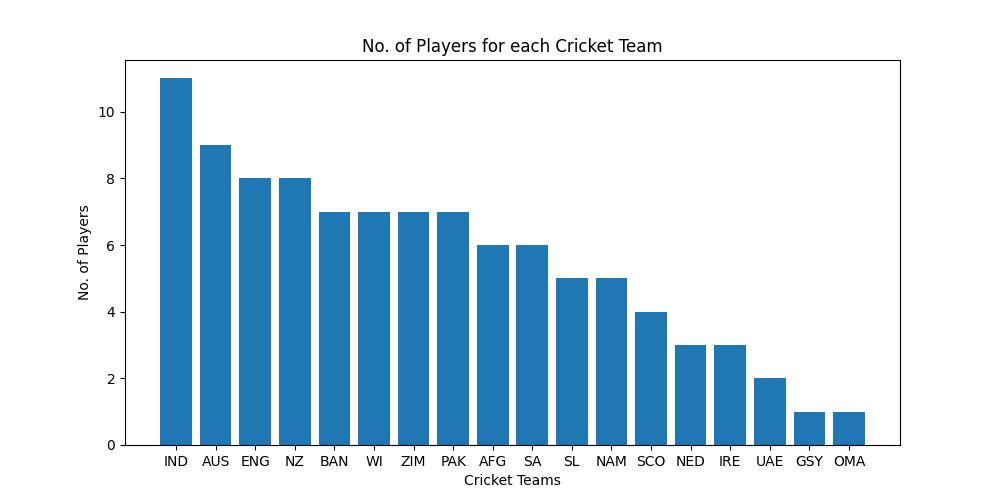
\includegraphics[scale=0.7]{t20i_bowling-1}
                \vspace{1em}\\
                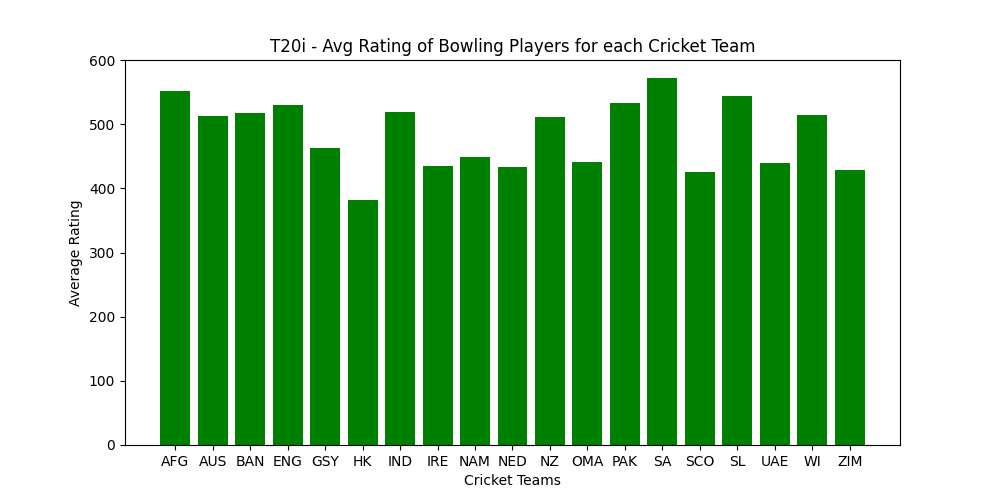
\includegraphics[scale=0.7]{t20i_bowling-2}
            \subsection{All-Rounder}\label{subsec:all-rounder1}
                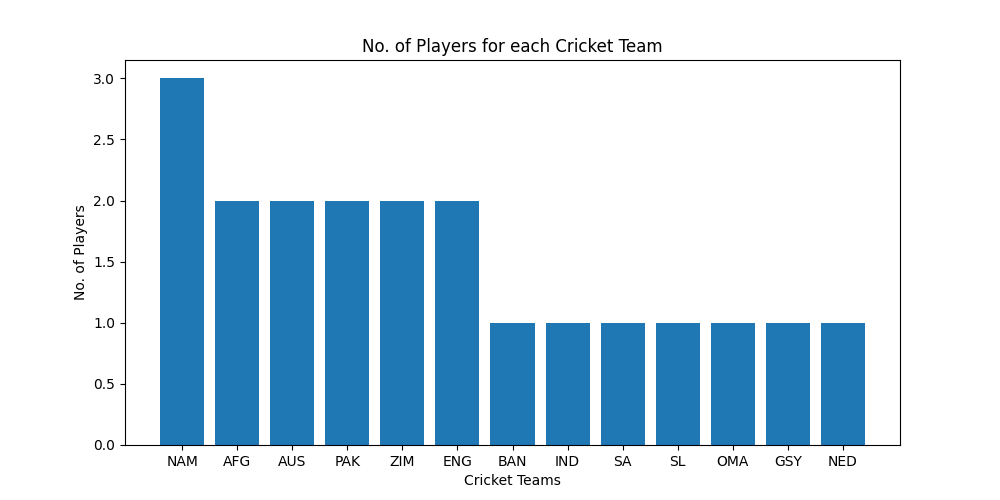
\includegraphics[scale=0.7]{t20i_all-rounder-1}
                \vspace{1em}\\
                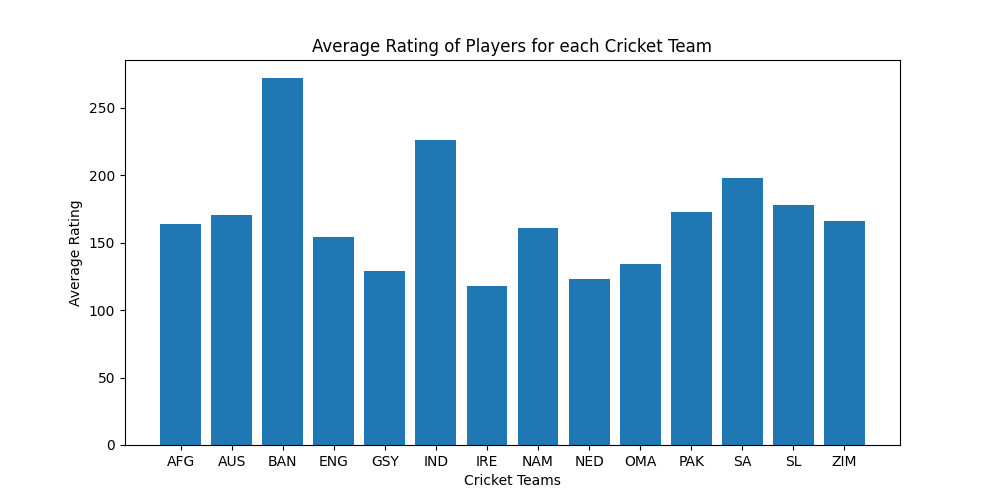
\includegraphics[scale=0.7]{t20i_all-rounder-2}

        \vspace{2em}

        \section{ODI Format}\label{sec:odi-format}
            \subsection{Batting}\label{subsec:batting2}
                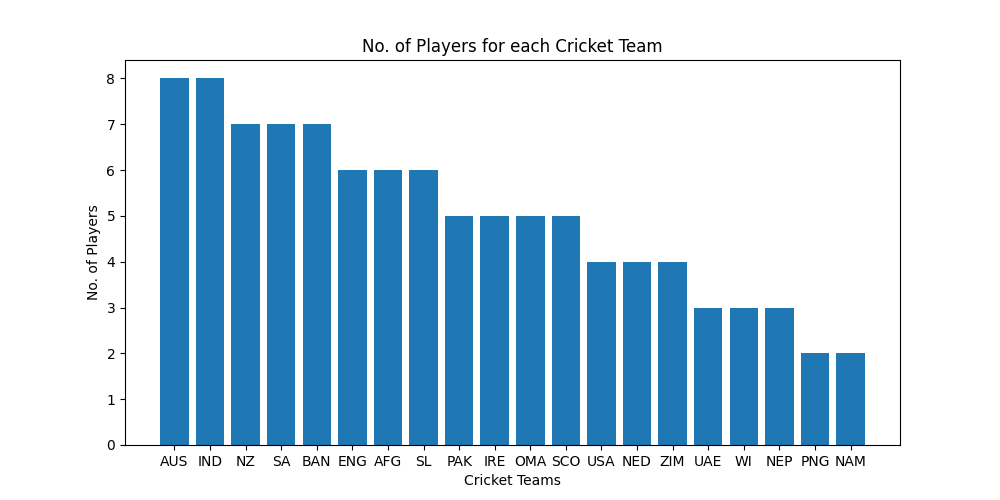
\includegraphics[scale=0.7]{odi_batting-1}
                \vspace{1em}\\
                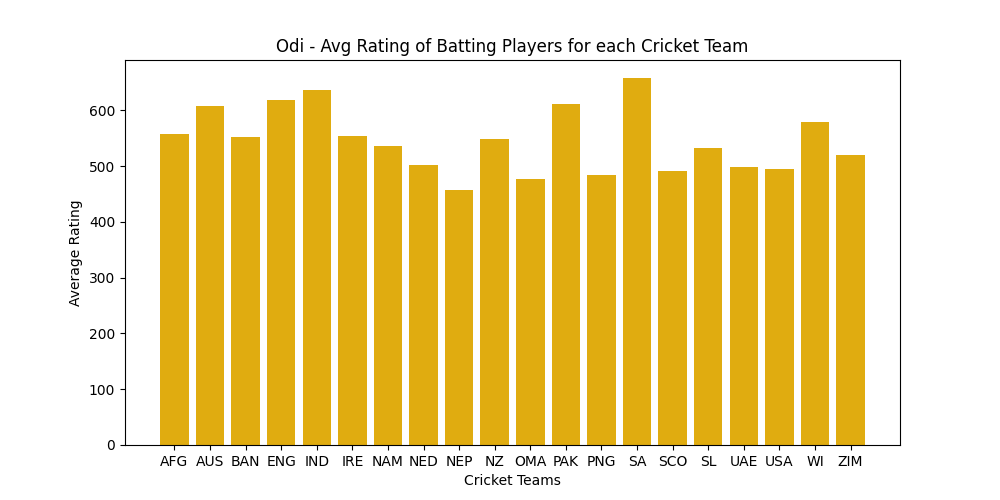
\includegraphics[scale=0.7]{odi_batting-2}
            \subsection{Bowling}\label{subsec:bowling2}
                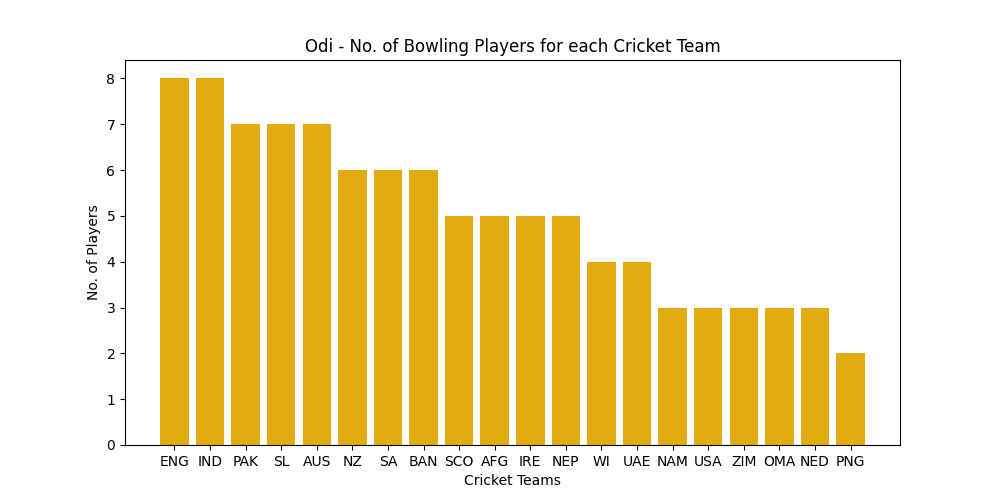
\includegraphics[scale=0.7]{odi_bowling-1}
                \vspace{1em}\\
                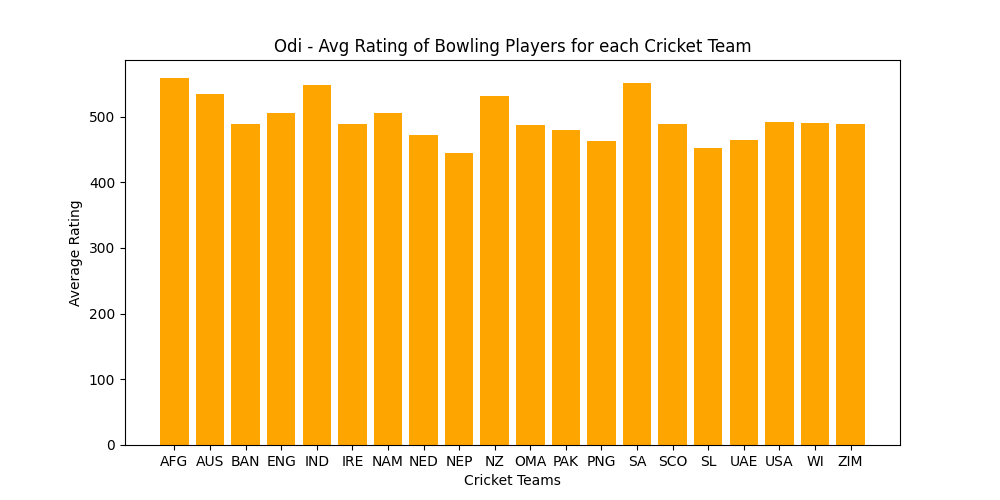
\includegraphics[scale=0.7]{odi_bowling-2}
            \subsection{All-Rounder}\label{subsec:all-rounder2}
                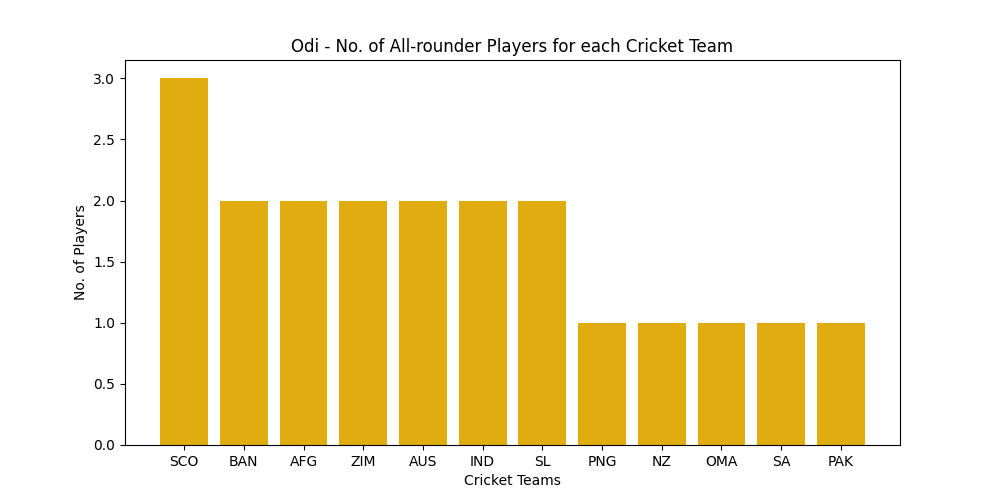
\includegraphics[scale=0.7]{odi_all-rounder-1}
                \vspace{1em}\\
                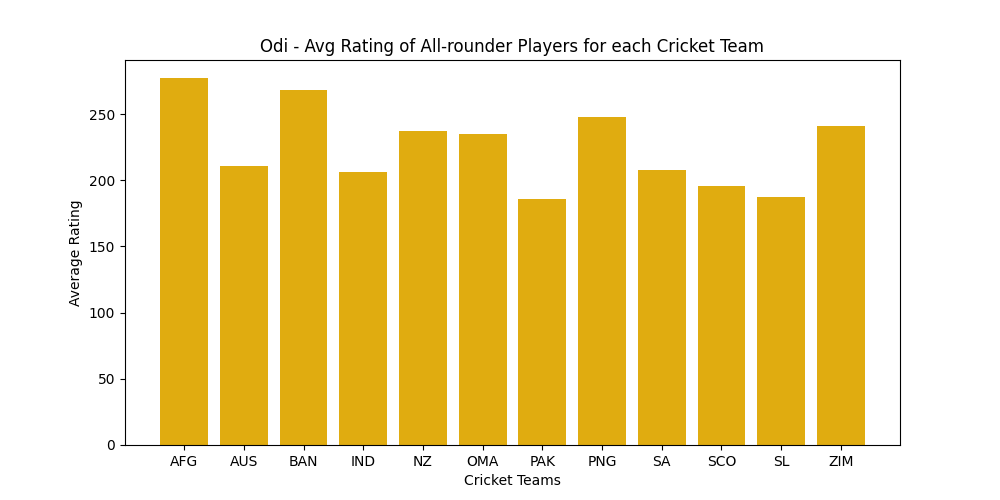
\includegraphics[scale=0.7]{odi_all-rounder-2}

        \vspace{2em}

        \section{Test Format}\label{sec:test-format}
            \subsection{Batting}\label{subsec:batting3}
                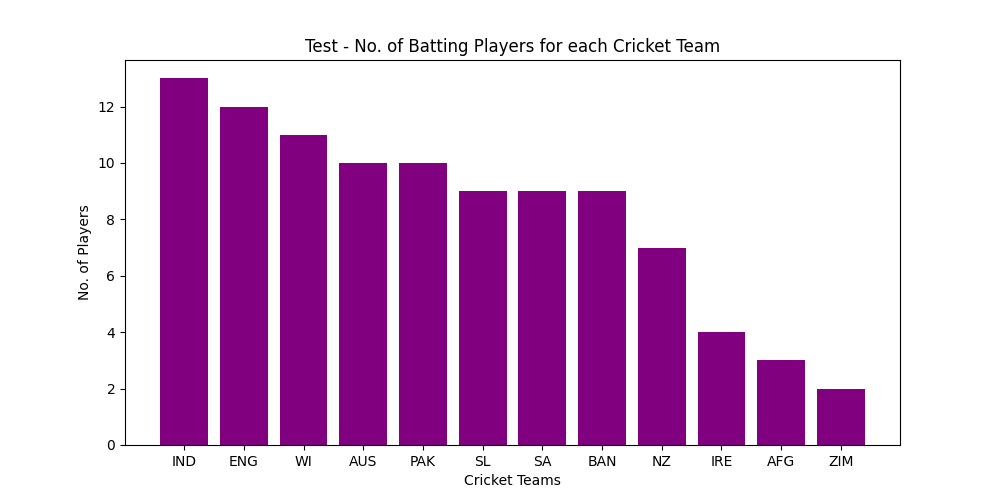
\includegraphics[scale=0.7]{test_batting-1}
                \vspace{1em}\\
                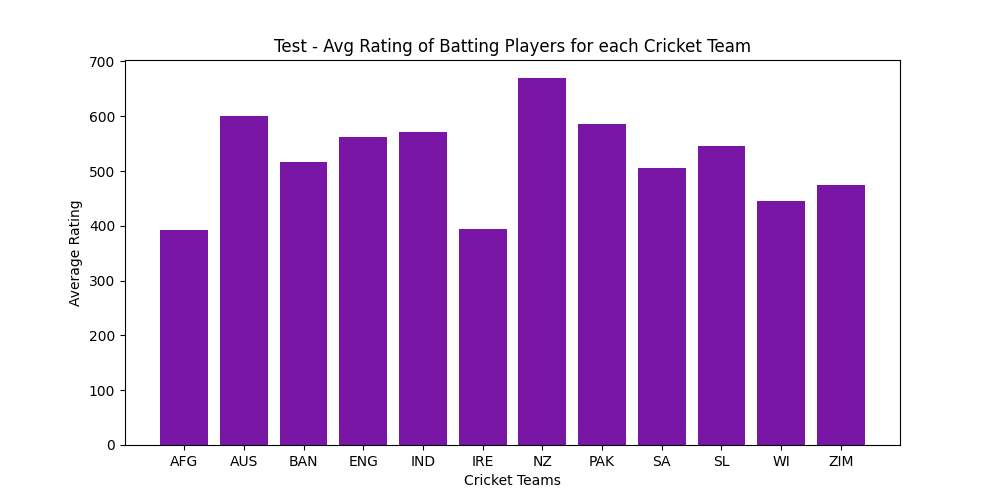
\includegraphics[scale=0.7]{test_batting-2}
            \subsection{Bowling}\label{subsec:bowling3}
                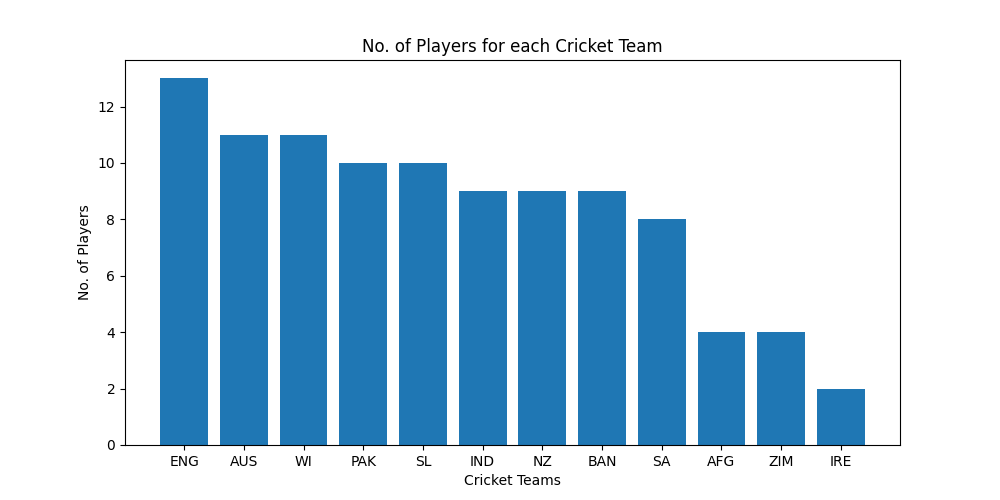
\includegraphics[scale=0.7]{test_bowling-1}
                \vspace{1em}\\
                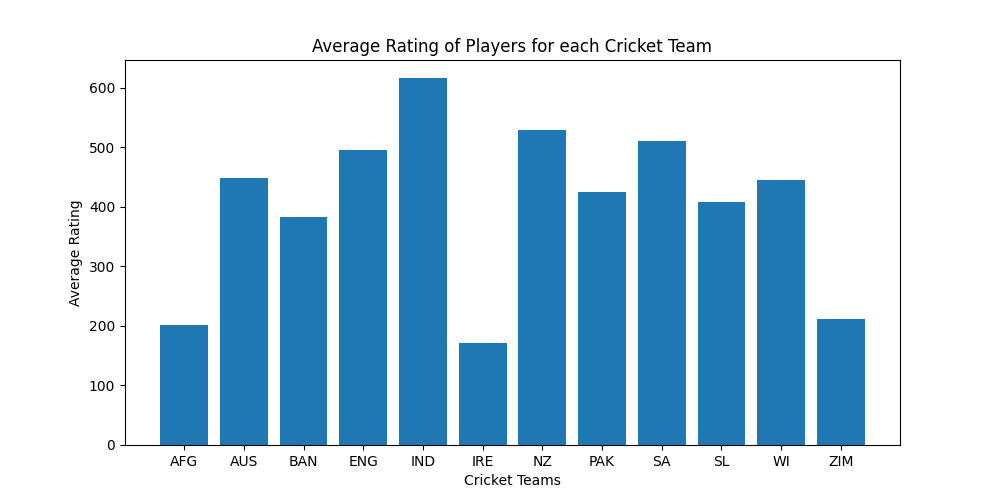
\includegraphics[scale=0.7]{test_bowling-2}
            \subsection{All-Rounder}\label{subsec:all-rounder3}
                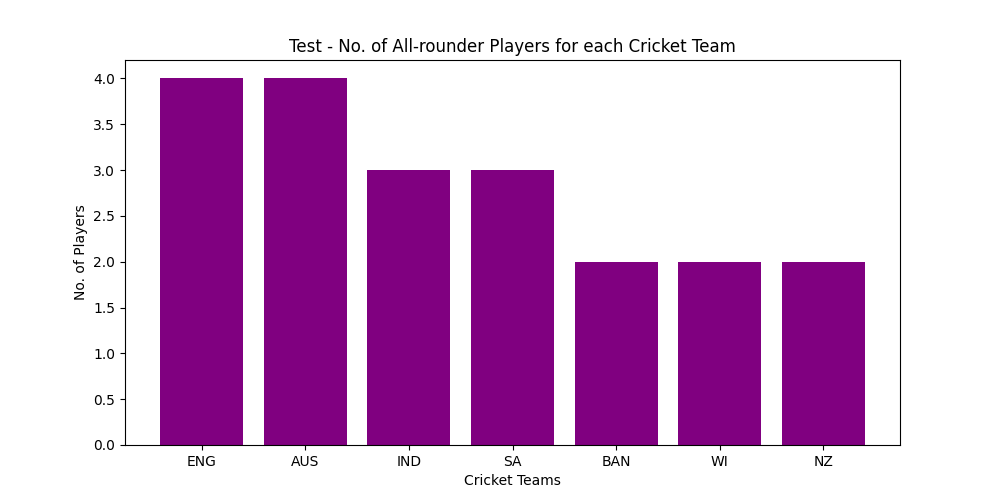
\includegraphics[scale=0.7]{test_all-rounder-1}
                \vspace{1em}\\
                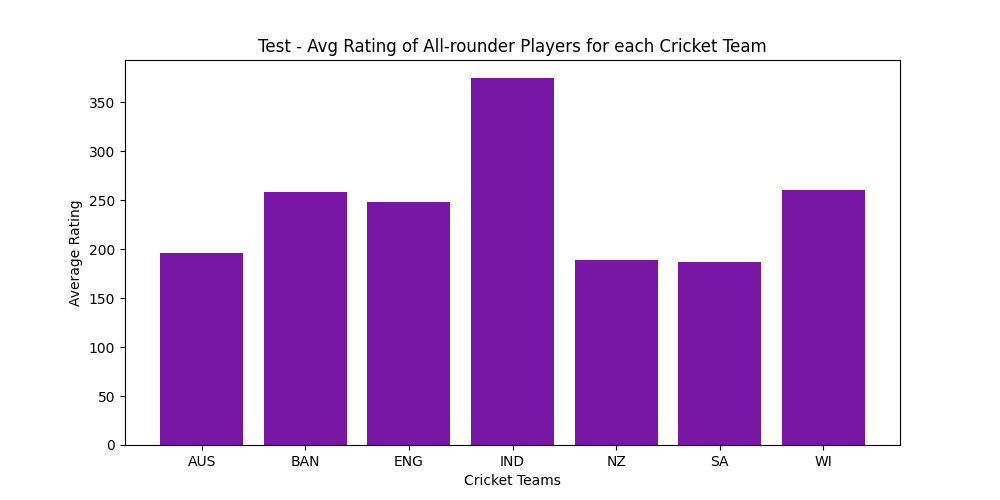
\includegraphics[scale=0.7]{test_all-rounder-2}
\end{normalsize}

\end{document}
